\documentclass[../main.tex]{subfiles}
\begin{document}

\todo{artifacts, hypothesis}

\subsection{solc-version-testset}
ABI v2 moves the majority of the interface code from the start to the end of the code compared to v1.

Optimization changes the how the ABI jump table is realized, solely causing significant changes for domain independent similarity measures.

Optimizations with high runs settings lead to a heavy reliance on storage operations, and causes a dramatically increase in overall code length.

Version changes are comparably smaller, but the default ABI encoding changed from v1 to v2 with solc version 0.8.0.

\todo{how do I know this?}

\subsection{JUMP-Hash}
Considering its simplicity it performs surprisingly well in separating contracts from different groups, partially due to the fact that the number of JUMPI opcodes has a very high f-statistic value.

It correlates strongly with NCD, wich seams to be more robust to optimization changes, but comparisons take 30 times longer and JUMP-Hash separates groups more sharply.

\todo{sharply?}
\todo{How do I know this?}

The nativ Levenshtein implementation used for comparison is the fastest out of all hash similarities used in this work. Only Jaccard applied to the much shorter Fourbyte signature sets is faster.

\todo{infestigate clusters within groups}

\subsection{Bytebag}
Combined with skeletonization and opcode filtering Bytebag performs better than ssdeep in some scenarios.

\subsection{LZJD parameters}

\csvreader[
  tabular=r|ll,
  table head= & Measure & Separation\\\hline,
  head to column names]{csv/lzjd_all_separation.csv}{}{\thecsvrow & \measure & \separation}

%\csvautotabular{../csv/lzjd_all_separation.csv}

\subsection{ssdeep variants}

\subsection{F-Stat filter}

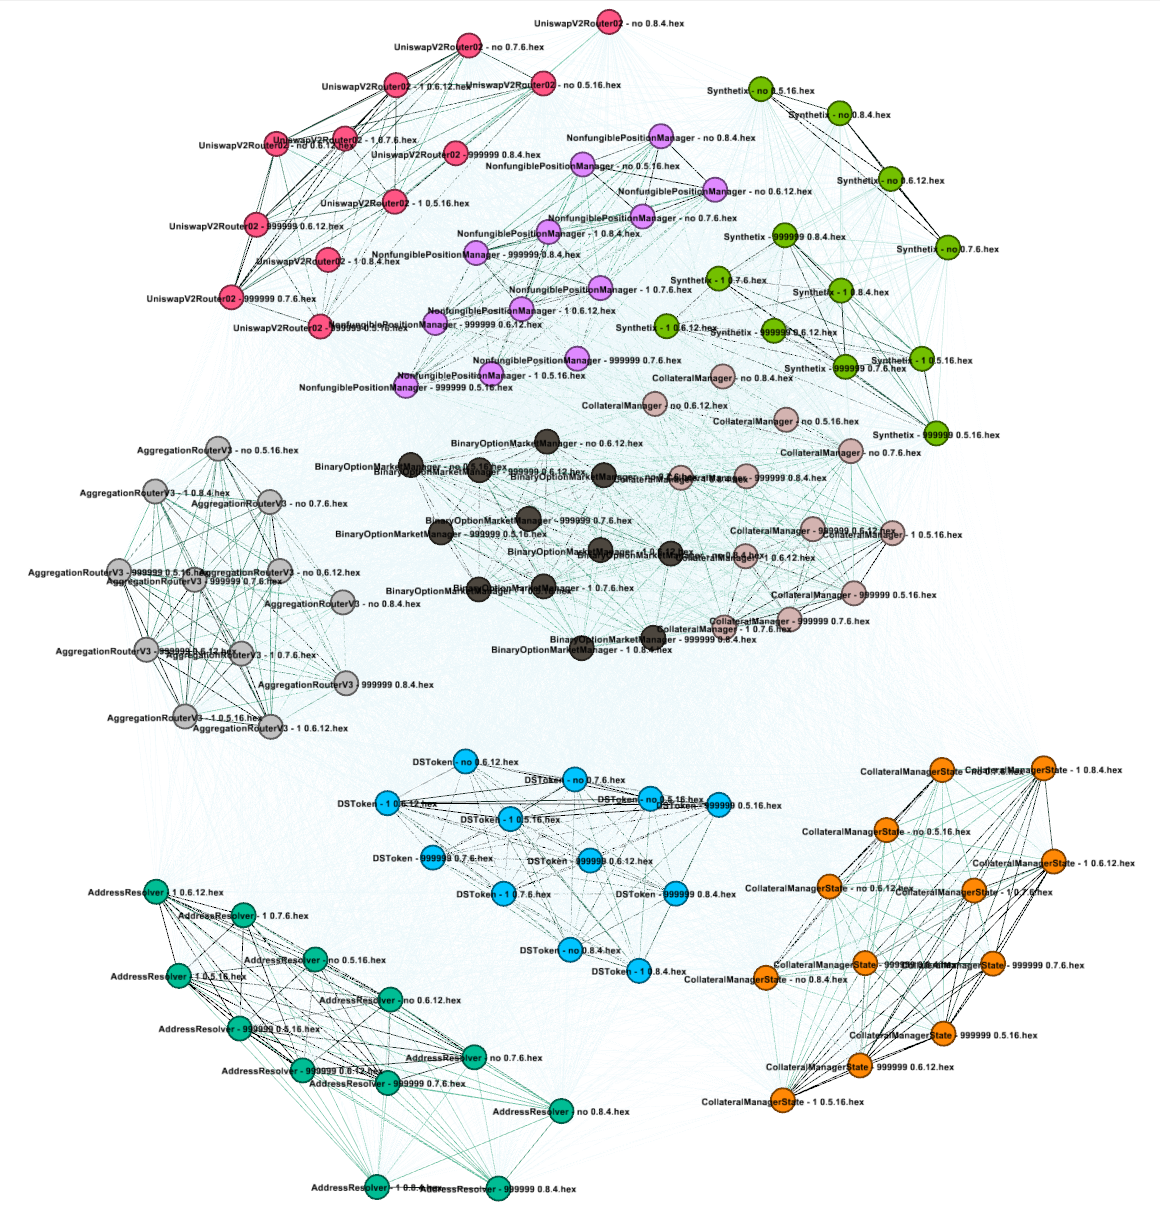
\includegraphics[width=\linewidth]{clustering_result_many_solc_versions_byteBag_significant_only_2021-06-06_163755.png}

\end{document}
